\documentclass[sigconf]{acmart}
\setcopyright{none}
\settopmatter{printacmref=false,printfolios=false}
\renewcommand\footnotetextcopyrightpermission[1]{}
\acmDOI{}
\acmISBN{}
\acmConference{}{}{}
\pagestyle{plain}
\fancyhead{}
\usepackage{booktabs}
\usepackage{listings}
\lstset{language=SQL,basicstyle=\ttfamily\scriptsize,breaklines=true,columns=fullflexible,keepspaces=true,showstringspaces=false,aboveskip=3pt,belowskip=3pt}
\newcommand{\repolink}{\url{https://github.com/MohamedKhalidmk/TRIAD}}

\begin{document}
\title{TRIAD: A Relational Model of Clinical Assertions}
\titlenote{Code, data, setup instructions, license and AI review log: \repolink.}
\author{Asish A. George}
\affiliation{\institution{University of Victoria}\city{Victoria}\state{BC}\country{Canada}}
\email{asishgeorge@uvic.ca}
\author{Mohamed Khaled}
\affiliation{\institution{University of Victoria}\city{Victoria}\state{BC}\country{Canada}}
\email{mabuela@uvic.ca}

\begin{abstract}
Clinical records are written by many people over years, and their facts change, yet a chart that stores only values cannot tell a correction from a contradiction. We map the TRIAD entity-relationship (ER) model to 29 relations in SQLite. Every clinical fact is an assertion carried by a message, issued by a staff member or the patient, and linked to the earlier assertion it supersedes, so the current fact is the one nothing supersedes. Keys and 11 triggers enforce this: assertions are append-only, and each entry has one current assertion. A web application demonstrates retrieval, insertion, update and deletion on Synthea data. Code: \repolink.
\end{abstract}

\keywords{Clinical records, relational data modeling, SQLite, SQL, provenance, data integrity}
\maketitle

\begin{figure*}[t]
\centering
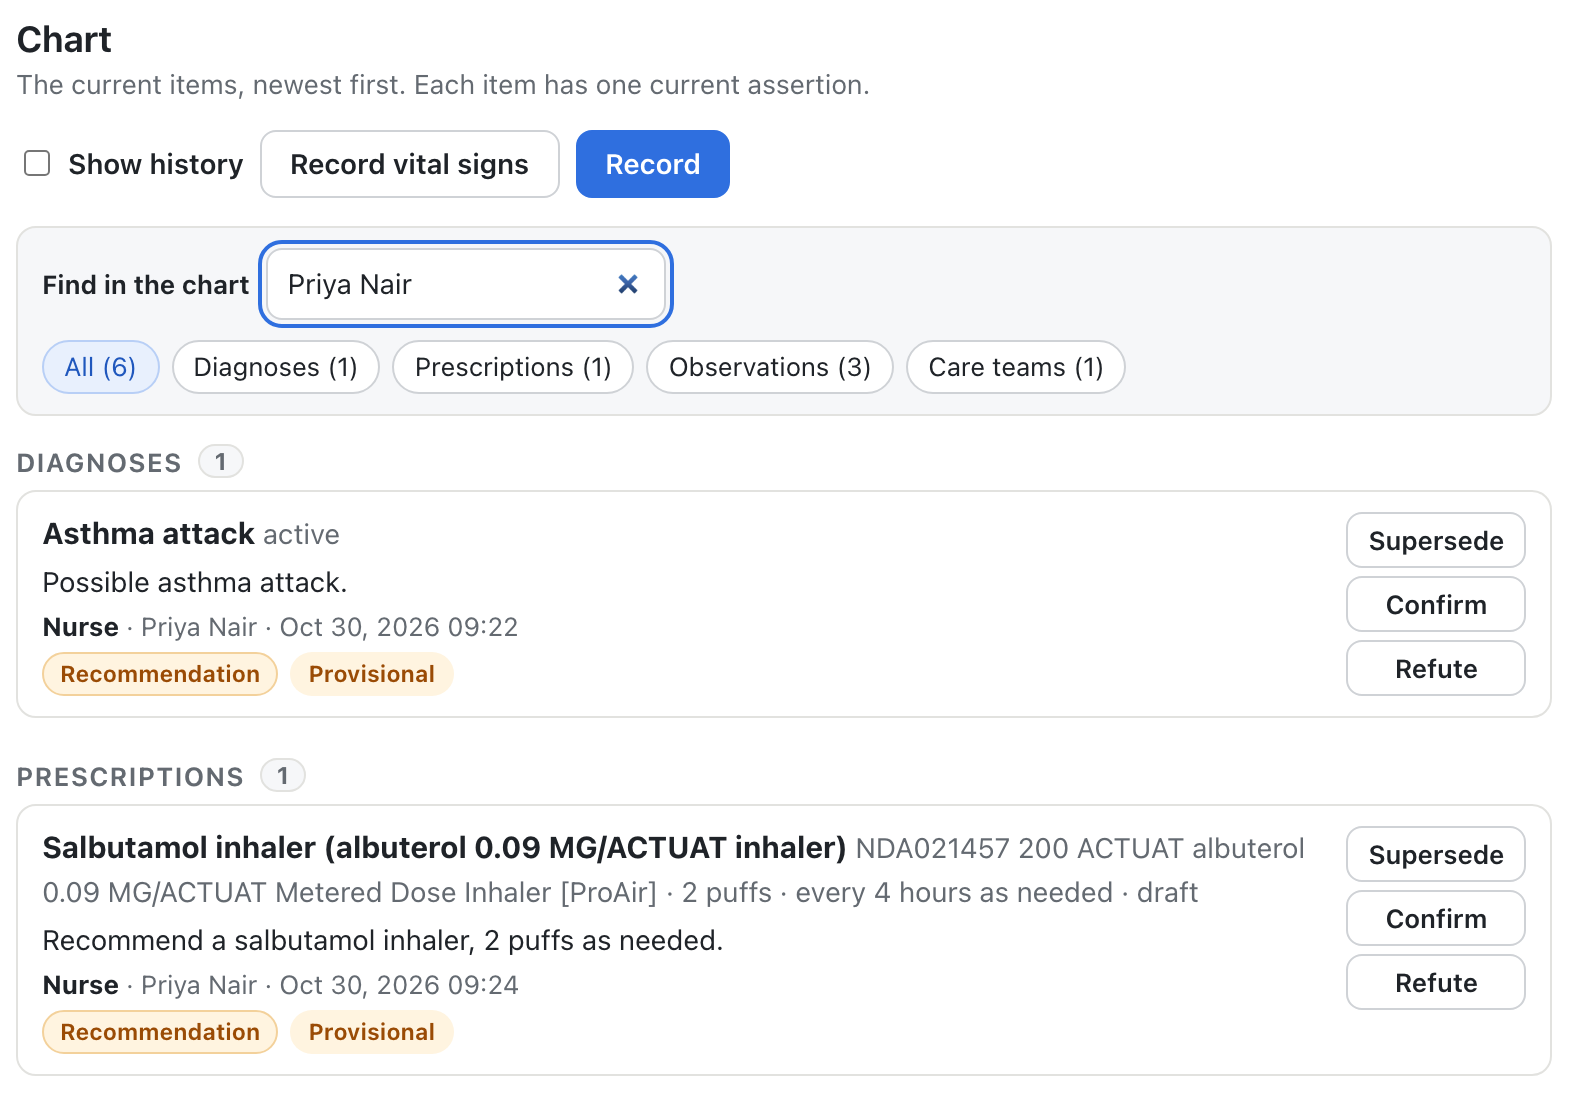
\includegraphics[width=.32\textwidth,height=42mm,keepaspectratio]{figures/03_nurse_triage_record.png}\hfill
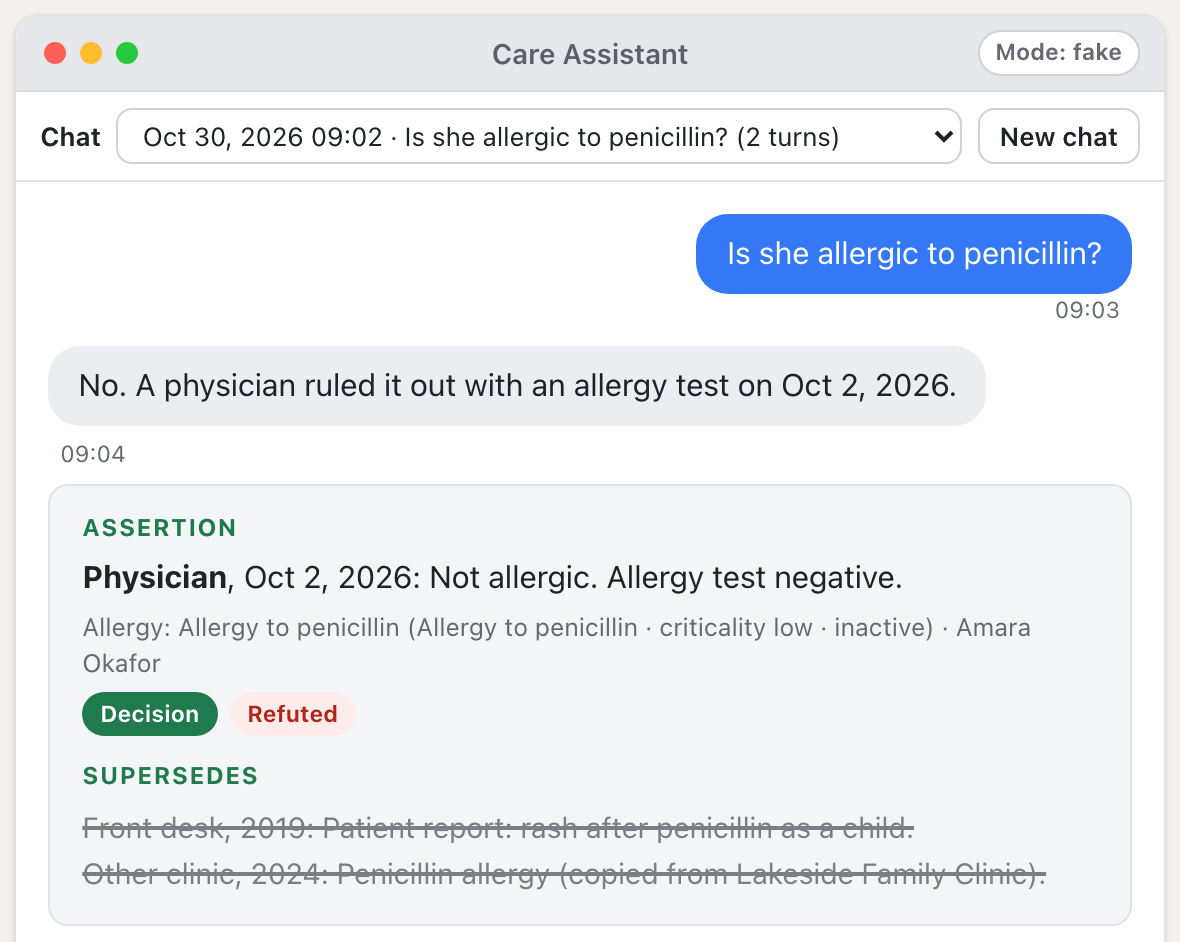
\includegraphics[width=.32\textwidth,height=42mm,keepaspectratio]{figures/01_doctor_slide_answer.png}\hfill
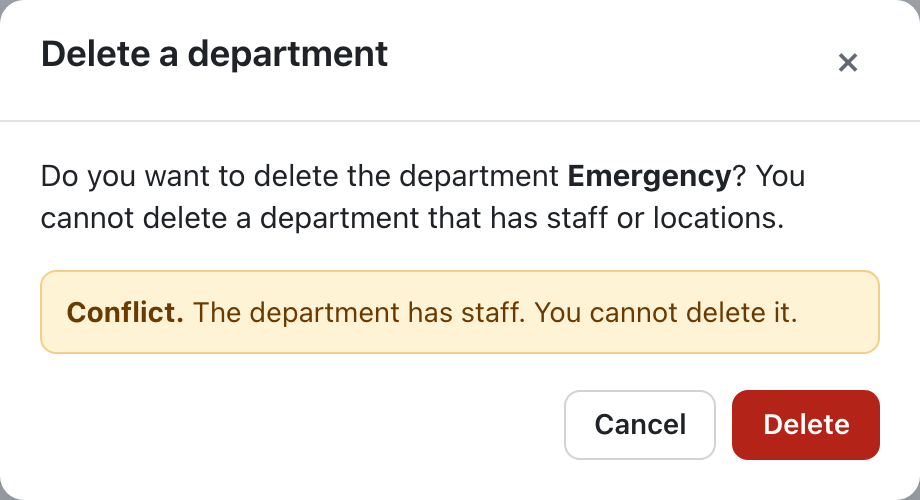
\includegraphics[width=.32\textwidth,height=42mm,keepaspectratio]{figures/09_moa_directory_409.png}
\caption{User interface. Left: a chart search finds the nurse's triage records. Middle: the penicillin answer cites the doctor's 2026 assertion and the superseded 2019 and 2024 claims (Q2). Right: deleting a department that has staff is refused.}
\label{fig:ui}
\end{figure*}

\section{Problem Definition}
Physicians spend about 49\% of their office day on records and desk work~\cite{sinsky2016}, much of it piecing together facts that changed. In 2019 a patient tells the front desk she had a rash after penicillin as a child, and the medical office assistant (MOA) records a penicillin allergy. In 2024 another clinic's record is copied in, repeating it. In 2026 an allergy test is negative, and the doctor rules the allergy out. A chart that stores only values still shows the penicillin banner: the correction looks like a contradiction, and a person, or an artificial intelligence (AI) assistant, must read every note to find what is true now.

\textbf{Information need.} For every clinical entry, return the current assertion (the one nothing supersedes), who issued it, through which message and when, and the chain of assertions it replaced. The schema must enforce this with keys and triggers, not by convention.

\section{Proposed Relational Model}\label{sec:model}
The ER diagram, revised after the Milestone~2 feedback (richer attributes, Staff \emph{issues} Message, Assertion weak on Message, Visit no longer weak), maps to 29 relations using the course's ER-to-relational rules. Every relation has an autogenerated \texttt{Id}; every ER key becomes a mandatory candidate key (CK), usually the Fast Healthcare Interoperability Resources (FHIR)~\cite{fhir-r4} identifier pair. All relations are listed on page~3.
\begin{itemize}
\item \textbf{Multivalued attributes} become relations of their own, e.g.\ \texttt{StaffLanguage}.
\item \textbf{Many-to-one} relationships put the foreign key (FK) on the many side, e.g.\ \texttt{Visit.PatientId}, mandatory.
\item \textbf{Many-to-many} relationships become relations with both FKs: \texttt{WorksIn} and \texttt{VisitLocation}.
\item \textbf{One-to-one} \emph{Supersedes} is a nullable FK, \texttt{SupersedesId} on \texttt{Assertion}, made a CK, so no assertion is superseded twice.
\item \textbf{Weak entities}: \texttt{Assertion} is owned by \texttt{Message}, with CK (\texttt{MessageId}, \texttt{Seq}).
\item \textbf{IS-A} uses one relation per parent and per child (Staff: Doctor, Nurse, MOA; ClinicalEntry: eight subtypes). The child's FK is the pair (\texttt{StaffId}, \texttt{Role}) with a CHECK on \texttt{Role}, so a Nurse row cannot point at a Doctor.
\end{itemize}
\textbf{The core.} A staff member issues a \texttt{Message}; a message from the patient has no issuer (\texttt{Origin = 'Patient'}). A message contains assertions; each is about one \texttt{ClinicalEntry} and may supersede one earlier assertion. Triggers enforce what keys cannot: assertions are append-only, a superseded assertion is older and about the same patient, and each entry has at most one current assertion.

\section{Relational Operations}\label{sec:operations}
Structured query language (SQL) script \texttt{01\_create\_\allowbreak tables.sql} creates the 29 tables and 11 triggers; \texttt{02\_insert\_seed.sql} fills every table. A loader also imports the 112 Synthea~\cite{synthea} patients and our curated FHIR bundle (113 patients in all, 5,090 visits, 57,022 assertions). Foreign keys are enforced with \texttt{PRAGMA foreign\_keys = ON}.

\subsection{SELECT}
\textbf{Q1, what is true now}, returns every assertion that nothing supersedes, with its entry and author (8 rows for the seed patient):
\par\noindent\begin{minipage}{\columnwidth}\begin{lstlisting}
SELECT e.Category, e.Display, a.Verification,
       COALESCE(s.Name, 'Patient') AS Author, a.Statement
FROM Patient p JOIN Visit v ON v.PatientId = p.Id
JOIN ClinicalEntry e ON e.VisitId = v.Id
JOIN Assertion a ON a.ClinicalEntryId = e.Id
JOIN Message m ON m.Id = a.MessageId LEFT JOIN Staff s ON s.Id = m.StaffId
WHERE p.Name = 'Elena Marsh' AND p.DateOfBirth = '1971-05-14'
  AND NOT EXISTS (SELECT 1 FROM Assertion n WHERE n.SupersedesId = a.Id);
\end{lstlisting}\end{minipage}\par
\textbf{Q2, the revision chain}, follows \emph{Supersedes} back from the current penicillin assertion: three rows, 2026, 2024, then 2019.
\par\noindent\begin{minipage}{\columnwidth}\begin{lstlisting}
WITH RECURSIVE chain (Id, SupersedesId, Depth) AS (
  SELECT a.Id, a.SupersedesId, 0 FROM Assertion a
  JOIN Allergy al ON al.ClinicalEntryId = a.ClinicalEntryId
  JOIN ClinicalEntry e ON e.Id = a.ClinicalEntryId
  JOIN Visit v ON v.Id = e.VisitId JOIN Patient p ON p.Id = v.PatientId
  WHERE p.Name = 'Elena Marsh' AND p.DateOfBirth = '1971-05-14'
    AND lower(al.Substance) LIKE '%penicillin%'
    AND NOT EXISTS (SELECT 1 FROM Assertion n WHERE n.SupersedesId = a.Id)
  UNION ALL
  SELECT a.Id, a.SupersedesId, c.Depth + 1
  FROM Assertion a JOIN chain c ON a.Id = c.SupersedesId)
SELECT c.Depth, date(a.AssertedAt), a.Verification, a.Statement
FROM chain c JOIN Assertion a ON a.Id = c.Id ORDER BY c.Depth;
\end{lstlisting}\end{minipage}\par
\textbf{Q8} aggregates over the IS-A: staff per department and role (13 rows; Cardiology has one doctor, one MOA and three nurses).
\par\noindent\begin{minipage}{\columnwidth}\begin{lstlisting}
SELECT d.Name, s.Role, COUNT(*) AS Staff,
       SUM(n.Designation = 'RN') AS RegisteredNurses
FROM Department d JOIN WorksIn w ON w.DepartmentId = d.Id
JOIN Staff s ON s.Id = w.StaffId LEFT JOIN Nurse n ON n.StaffId = s.Id
GROUP BY d.Id, s.Role;
\end{lstlisting}\end{minipage}\par

\subsection{INSERT, UPDATE and DELETE}
An update and an FK-safe delete:
\par\noindent\begin{minipage}{\columnwidth}\begin{lstlisting}
UPDATE Patient SET PhoneNumber = '+1-508-555-0199'
WHERE Name = 'Elena Marsh' AND DateOfBirth = '1971-05-14';
DELETE FROM Location WHERE IdentifierValue = 'STORE-OLD'
  AND NOT EXISTS (SELECT 1 FROM VisitLocation vl
                  WHERE vl.LocationId = Location.Id);
\end{lstlisting}\end{minipage}\par
A clinical fact is never overwritten. A patient report through the app inserts a \texttt{Message} with no issuer and an \texttt{Assertion} that supersedes the current one; the old one stays (script 04, step~5):
\par\noindent\begin{minipage}{\columnwidth}\begin{lstlisting}
INSERT INTO Message (IdentifierSystem, IdentifierValue, StaffId, Channel,
  Origin, SentAt, Text) VALUES ('https://triad.example/fhir/sid/message',
  'MSG-ELENA-APP-0001', NULL, 'App', 'Patient', '2026-10-30T08:30:00-04:00',
  'I take amlodipine every morning.');
INSERT INTO Assertion (MessageId, Seq, ClinicalEntryId, SupersedesId,
  AssertedAt, Intent, Source, Verification, Statement)
SELECT last_insert_rowid(), 1, a.ClinicalEntryId, a.Id,
  '2026-10-30T08:30:00-04:00', 'Report', 'Human', 'Unconfirmed',
  'I take amlodipine every morning.'
FROM Assertion a JOIN ClinicalEntry e ON e.Id = a.ClinicalEntryId
WHERE e.IdentifierValue = 'MedicationRequest/mr-elena-amlodipine'
  AND NOT EXISTS (SELECT 1 FROM Assertion n WHERE n.SupersedesId = a.Id);
\end{lstlisting}\end{minipage}\par
Changing an assertion in place fails (\emph{Assertion is append-only}), as do all 26 statements of \texttt{05\_constraint\_\allowbreak violations.sql}.

\begin{figure}[t]
\centering
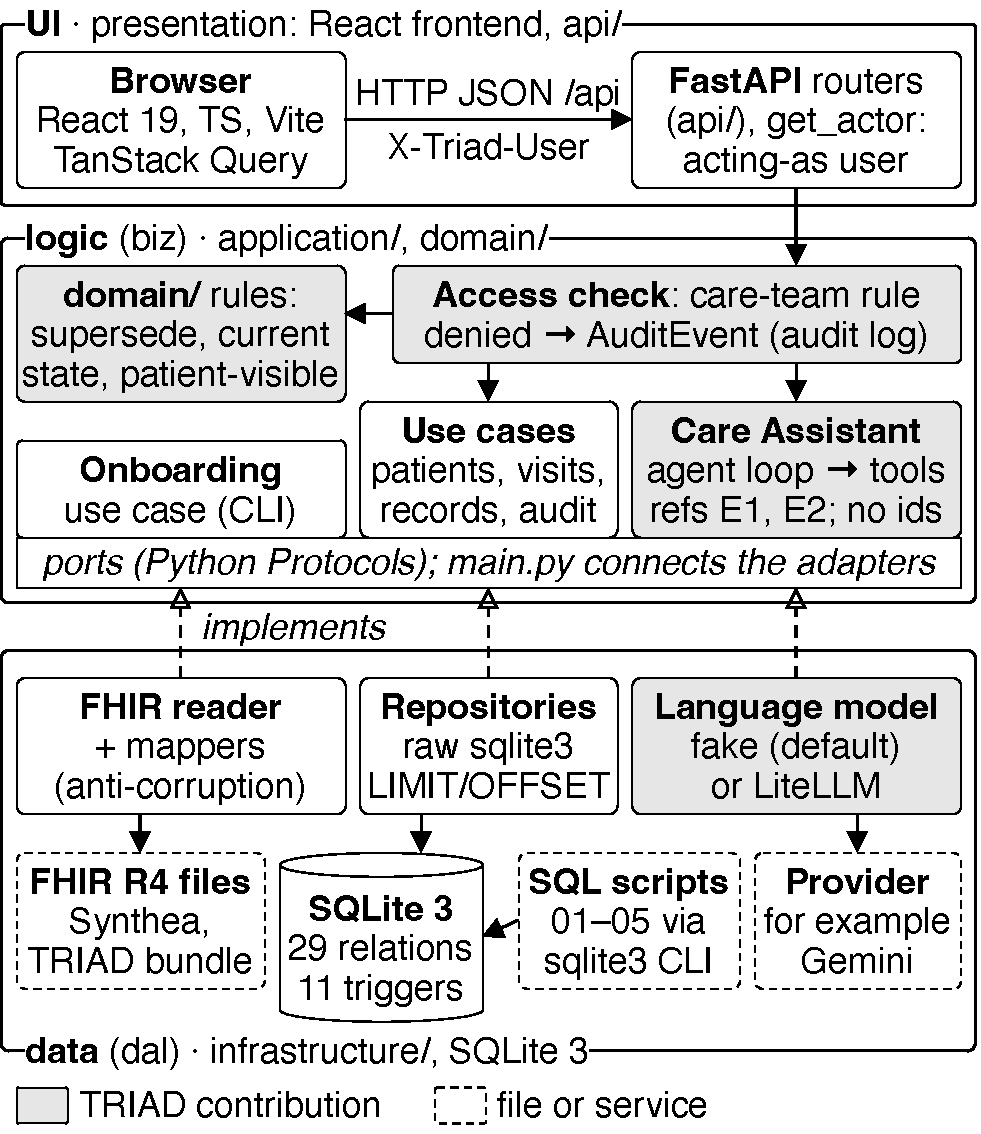
\includegraphics[width=.64\columnwidth]{figures/architecture.pdf}
\caption{Architecture. Grey boxes are TRIAD's contribution.}
\label{fig:arch}
\end{figure}



\section{Architecture and User Interface}
Figure~\ref{fig:arch} shows three layers. In the \emph{user interface}, a React application sends JavaScript Object Notation (JSON) requests to a FastAPI application programming interface (API); each request names the acting user (doctor, nurse, MOA or patient). The \emph{logic} layer holds the domain rules (supersede, current state, what a patient may see) and an access check: only the patient's care team may read a chart, and a denied attempt is written to \texttt{AuditEvent}. The \emph{data} layer issues plain SQL to SQLite. Figure~\ref{fig:ui} shows the operations.

\section{Reproducibility and Evaluation}
\texttt{src/scripts/quickstart.sh} checks the prerequisites, installs pinned packages, builds the frontend and the database, runs the tests and serves the application; the chat uses a fake large language model (LLM) by default, so no key or network is needed. On a fresh clone, the application served in about 25\,s, the five scripts ran with no FK violations, and all 422 tests passed.

\textbf{AI use and critique.} Claude Code~\cite{claudecode} generated most of the code, SQL and tests; \texttt{doc/ai\_review\_log.md} records what we checked. The AI dropped our no-loops rule in the ER diagram to mirror FHIR, proposed one visit per version of a fact (we rejected it), and wrote code that passed type checks yet silently ignored a phone update; only an end-to-end test caught it. These errors fall where the model decided alone. A language model recognizes and continues patterns: given our design and examples, it was reliable; asked to decide without them, it guessed. We treat it as a junior engineer, not the architect. Claude also helped draft this report; we checked every number and query.

\bibliographystyle{ACM-Reference-Format}
\bibliography{bibliography}

\clearpage
\onecolumn
\section*{Relations and Constraints}
\footnotesize
Every relation has an autogenerated surrogate key \underline{Id} (INTEGER PRIMARY KEY AUTOINCREMENT). CK = candidate key, enforced by UNIQUE and NOT NULL; every ER key becomes a CK. FK = foreign key to the target's Id, with no cascading delete. ? marks an optional (nullable) attribute; all others are mandatory. Ident = (IdentifierSystem, IdentifierValue), the FHIR identifier. Addr = Street?, City?, Region?, PostalCode?, Country?. ``As in 14'' = CK ClinicalEntryId; FK (ClinicalEntryId, Category) $\to$ ClinicalEntry(Id, Category).
\begin{enumerate}\setlength{\itemsep}{0pt}\setlength{\parskip}{0pt}
\item Department(\underline{Id}, Ident, Name, Type?, PhoneNumber?, Email?, Addr). CK Ident.
\item Location(\underline{Id}, Ident, Name, Type?, PhysicalType?, PhoneNumber?, Addr). CK Ident.
\item Staff(\underline{Id}, Ident, Name, Sex?, Email?, PhoneNumber?, Active, Role). CK Ident; CK (Id, Role) for the subtypes. Role $\in$ \{Doctor, Nurse, MOA\}; Active $\in$ \{0, 1\}.
\item StaffLanguage(\underline{Id}, StaffId, Language). CK (StaffId, Language); FK StaffId $\to$ Staff.
\item WorksIn(\underline{Id}, StaffId, DepartmentId, RoleCode, Specialty?, StartDate?, EndDate?). CK (StaffId, DepartmentId, RoleCode); FK StaffId $\to$ Staff; FK DepartmentId $\to$ Department. EndDate $\ge$ StartDate.
\item Doctor(\underline{Id}, StaffId, Role, LicenseNumber?, Qualification?). CK StaffId; FK (StaffId, Role) $\to$ Staff(Id, Role). Role = Doctor.
\item Nurse(\underline{Id}, StaffId, Role, LicenseNumber?, Designation). CK StaffId; FK (StaffId, Role) $\to$ Staff(Id, Role). Role = Nurse; Designation $\in$ \{RN, LPN, RPN, NP\}.
\item MOA(\underline{Id}, StaffId, Role, CertificationNumber?, Desk, PhoneExtension?). CK StaffId; FK (StaffId, Role) $\to$ Staff(Id, Role). Role = MOA.
\item Patient(\underline{Id}, Name, DateOfBirth, Sex, PhoneNumber?, Addr). CK (Name, DateOfBirth). Sex $\in$ \{female, male, other, unknown\}.
\item PatientIdentifier(\underline{Id}, PatientId, System, Value). CK (System, Value); FK PatientId $\to$ Patient.
\item Visit(\underline{Id}, Ident, PatientId, Class, Type?, Reason?, StartDate, EndDate?). CK Ident; FK PatientId $\to$ Patient (Has). Class $\in$ \{AMB, EMER, IMP, HH, VR\}; EndDate $\ge$ StartDate.
\item VisitLocation(\underline{Id}, VisitId, LocationId, StartDate, EndDate?). CK (VisitId, LocationId, StartDate); FK VisitId $\to$ Visit; FK LocationId $\to$ Location (TakesPlaceIn). EndDate $\ge$ StartDate.
\item ClinicalEntry(\underline{Id}, Ident, VisitId, Category, Code, CodeSystem, Display, Text?, RecordedAt). CK Ident; CK (Id, Category) for the subtypes; FK VisitId $\to$ Visit (During, total). Category is one of the eight subtypes.
\item Diagnosis(\underline{Id}, ClinicalEntryId, Category, OnsetDate?, AbatementDate?, ClinicalStatus, Severity?). CK ClinicalEntryId; FK (ClinicalEntryId, Category) $\to$ ClinicalEntry(Id, Category). Category = Diagnosis.
\item Procedure(\underline{Id}, ClinicalEntryId, Category, PerformedDate, Outcome?). As in 14; Category = Procedure.
\item Allergy(\underline{Id}, ClinicalEntryId, Category, Substance, Type?, AllergyCategory?, Criticality?, ClinicalStatus?). As in 14; Category = Allergy.
\item Observation(\underline{Id}, ClinicalEntryId, Category, Value, Unit?). As in 14; Category = Observation.
\item LabOrder(\underline{Id}, ClinicalEntryId, Category, TestName, Priority, Specimen?). As in 14; Priority $\in$ \{routine, urgent, asap, stat\}.
\item LabReport(\underline{Id}, ClinicalEntryId, Category, IssuedDate, Conclusion?). As in 14; Category = LabReport.
\item Medication(\underline{Id}, Code, CodeSystem, Name, Form?, Manufacturer?). CK (Code, CodeSystem).
\item Prescription(\underline{Id}, ClinicalEntryId, Category, MedicationId, Dosage?, Frequency?, Status). As in 14; FK MedicationId $\to$ Medication (Prescribes).
\item CareTeam(\underline{Id}, ClinicalEntryId, Category, Name?, Status). As in 14; Status $\in$ \{proposed, active, suspended, inactive, entered-in-error\}.
\item CareTeamMember(\underline{Id}, CareTeamId, MemberSystem, MemberValue, Role?). CK (CareTeamId, MemberSystem, MemberValue); FK CareTeamId $\to$ CareTeam. The member must be a staff identifier (trigger).
\item Message(\underline{Id}, Ident, StaffId?, Channel, Origin, SentAt, Text). CK Ident; FK StaffId $\to$ Staff (Issues), optional. StaffId IS NOT NULL OR Origin = Patient.
\item Assertion(\underline{Id}, MessageId, Seq, ClinicalEntryId, SupersedesId?, AssertedAt, Intent, Source, Verification, Statement). CK (MessageId, Seq) (weak entity); CK SupersedesId (optional, one-to-one); FK MessageId $\to$ Message (Contains); FK ClinicalEntryId $\to$ ClinicalEntry (About); FK SupersedesId $\to$ Assertion (Supersedes). SupersedesId $\ne$ Id; Intent, Source and Verification take fixed value sets.
\item ChatSession(\underline{Id}, Ident, UserRole, UserSystem, UserValue, SubjectName, SubjectDateOfBirth, StartedAt, Mode, Model?). CK Ident. Mode $\in$ \{rules, fake, llm\}; user and subject are stored as values.
\item ChatTurn(\underline{Id}, ChatSessionId, Seq, ClientTurnId, Speaker, Text, CreatedAt). CK (ChatSessionId, Seq) (weak entity); CK (ChatSessionId, ClientTurnId); FK ChatSessionId $\to$ ChatSession (Includes). Speaker $\in$ \{User, Assistant\}.
\item Citation(\underline{Id}, ChatTurnId, AssertionId, Rank). CK (ChatTurnId, AssertionId); FK ChatTurnId $\to$ ChatTurn; FK AssertionId $\to$ Assertion (Cites). Rank $\ge$ 1.
\item AuditEvent(\underline{Id}, Ident, At, Action, Outcome, ActorRole, ActorSystem, ActorValue, SubjectName, SubjectDateOfBirth, Path, ChatTurnId?). CK Ident; FK ChatTurnId $\to$ ChatTurn (InTurn), optional. Outcome $\in$ \{Allowed, Denied\}; actor and subject are stored as values.
\end{enumerate}
\paragraph{Triggers (11 rules a CHECK cannot express).} Assertions are append-only: no UPDATE or DELETE; a correction is a new superseding assertion. A superseded assertion must be older and about the same patient. Each entry has at most one current assertion. All assertions in one message concern one patient. A care-team member must match a staff identifier. Only an assistant turn may cite, and only assertions about the chat's patient. Audit records are append-only, and an audit record tied to a chat turn must name that chat's patient. A patient's key (Name, DateOfBirth) cannot be updated, since the logs store it as a value.
\paragraph{Mapping assumptions.} Patients are identified by (Name, DateOfBirth), with external record numbers in PatientIdentifier. A message without a staff issuer comes from the patient. Chat and audit records keep the user and patient as values, so they stay correct when a row changes and add no loop to the ER diagram. Times are ISO 8601 text with an offset from Coordinated Universal Time (UTC).
\end{document}
